\documentclass[tikz,border=0pt]{standalone}
\usepackage{xcolor}
\usetikzlibrary{calc}
% Palette: Sam_Comm_final.png by eye, and the drones and raiders.
\definecolor{ink}{HTML}{3B2340}
\definecolor{sky}{HTML}{EFC46A}
\definecolor{skyhi}{HTML}{F5DA92}
\definecolor{skylow}{HTML}{E9B060}
\definecolor{cloud}{HTML}{F2D58A}
\definecolor{paper}{HTML}{FBEFD0}
\definecolor{cream}{HTML}{FFF6E0}
\definecolor{white}{HTML}{FFFFFF}
\definecolor{wallA}{HTML}{E88A73}
\definecolor{wallB}{HTML}{EE9F7E}
\definecolor{wallC}{HTML}{E47A7E}
\definecolor{wallD}{HTML}{F0B07E}
\definecolor{wallE}{HTML}{D9765F}
\definecolor{wallF}{HTML}{E99A8A}
\definecolor{greenA}{HTML}{8DBB7E}
\definecolor{greenB}{HTML}{6FA77A}
\definecolor{greenC}{HTML}{A9C97F}
\definecolor{greenD}{HTML}{5E9C6A}
\definecolor{greenE}{HTML}{4A8060}
\definecolor{sage}{HTML}{9DB98A}
\definecolor{sagedark}{HTML}{6F8F66}
\definecolor{sagelight}{HTML}{C2D6A6}
\definecolor{window}{HTML}{F6E7A0}
\definecolor{windark}{HTML}{8C5A64}
\definecolor{metal}{HTML}{8D9A93}
\definecolor{metaldark}{HTML}{5E6B66}
\definecolor{metallight}{HTML}{B9C4BC}
\definecolor{wood}{HTML}{B9835A}
\definecolor{wooddark}{HTML}{8C5A3C}
\definecolor{woodlight}{HTML}{D9A66F}
\definecolor{stone}{HTML}{E7C9A0}
\definecolor{stonedark}{HTML}{C9A47E}
\definecolor{concrete}{HTML}{D8C3A4}
\definecolor{concretedark}{HTML}{B8A084}
\definecolor{asphalt}{HTML}{8E7A86}
\definecolor{asphaltdark}{HTML}{6E5C68}
\definecolor{roadline}{HTML}{F6E7A0}
\definecolor{kerb}{HTML}{D8B48C}
\definecolor{red}{HTML}{E0483E}
\definecolor{redlight}{HTML}{F27A6A}
\definecolor{gold}{HTML}{FFB000}
\definecolor{goldlight}{HTML}{FFD54F}
\definecolor{teal}{HTML}{4FA3A0}
\definecolor{tealdark}{HTML}{3C8582}
\definecolor{magenta}{HTML}{FF2E88}
\definecolor{cyan}{HTML}{13CFE3}
\definecolor{violet}{HTML}{8A5BD6}
\definecolor{orange}{HTML}{F2803A}
\definecolor{pink}{HTML}{F48FB1}
\definecolor{glow}{HTML}{4FE6E0}
\definecolor{glowhi}{HTML}{C8FFF9}
\definecolor{hot}{HTML}{FF6A1A}
\definecolor{hothi}{HTML}{FFD07A}
\definecolor{armour}{HTML}{7E7A86}
\definecolor{armourdark}{HTML}{5A5466}
\definecolor{armourlight}{HTML}{A8A2B0}
\definecolor{wasp}{HTML}{E0A82E}
\definecolor{waspdark}{HTML}{B07E1A}
\definecolor{moth}{HTML}{F2E6C8}
\definecolor{mothdark}{HTML}{D2C09A}
\definecolor{hornet}{HTML}{3C8582}
\definecolor{hornetdark}{HTML}{2C6260}
\definecolor{warden}{HTML}{E47A7E}
\definecolor{wardendark}{HTML}{B85A62}
\definecolor{tick}{HTML}{8DBB7E}
\definecolor{tickdark}{HTML}{5E8A5A}
\definecolor{strider}{HTML}{D9765F}
\definecolor{striderdark}{HTML}{A8543F}
\definecolor{jacket}{HTML}{6FA77A}
\definecolor{jacketb}{HTML}{4FA3A0}
\definecolor{jacketc}{HTML}{E88A73}
\definecolor{jacketd}{HTML}{F0B07E}
\definecolor{skin}{HTML}{F2C49A}
\definecolor{skinb}{HTML}{C98C6A}
\definecolor{skinc}{HTML}{8C5A3C}
\definecolor{hair}{HTML}{3B2340}
\definecolor{goo}{HTML}{B6E35A}
\definecolor{goodark}{HTML}{7FB23A}
\newcommand{\Ink}{1.8pt}
\tikzset{inked/.style={draw=ink, line width=\Ink, line join=round, line cap=round}}
\begin{document}
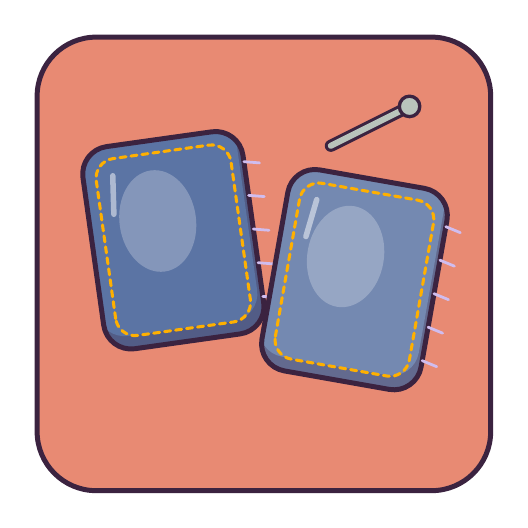
\begin{tikzpicture}
\clip (0,0) rectangle (6,6);
\fill[wallA] [rounded corners=0.75cm] (0.12,0.12) rectangle (5.88,5.88);
\begin{scope}\clip [rounded corners=0.75cm] (0.12,0.12) rectangle (5.88,5.88);
\begin{scope}[shift={(1.85,3.3)}, rotate=0, xscale=1.08, yscale=1.08]
\begin{scope}[shift={(0,0)}, rotate=8, xscale=1, yscale=1]
\begin{scope}\clip [rounded corners=0.35cm] (-0.95,-1.2) rectangle (0.95,1.2);
\fill[tealdark!60!violet!70!ink] [rounded corners=0.35cm] (-0.95,-1.2) rectangle (0.95,1.2);
\fill[tealdark!60!violet, shift={(-0.056,0.16)}] [rounded corners=0.35cm] (-0.95,-1.2) rectangle (0.95,1.2);
\end{scope}
\draw[inked] [rounded corners=0.35cm] (-0.95,-1.2) rectangle (0.95,1.2);
\draw[gold, line width=1.1pt, line cap=round, dash pattern=on 2.2pt off 1.8pt] [rounded corners=0.25cm] (-0.8,-1.05) rectangle (0.8,1.05);
\draw[white!60!violet, line width=1pt, line cap=round] (0.95,-0.8) -- (1.13,-0.84);
\draw[white!60!violet, line width=1pt, line cap=round] (0.95,-0.4) -- (1.13,-0.44);
\draw[white!60!violet, line width=1pt, line cap=round] (0.95,0) -- (1.13,-0.04);
\draw[white!60!violet, line width=1pt, line cap=round] (0.95,0.4) -- (1.13,0.36);
\draw[white!60!violet, line width=1pt, line cap=round] (0.95,0.8) -- (1.13,0.76);
\fill[white, opacity=0.25] (-0.15,0.25) ellipse (0.45 and 0.6);
\draw[white, line width=2pt, line cap=round, line join=round, opacity=0.5] plot[smooth, tension=0.6] coordinates {(-0.65,0.4) (-0.6,0.85)};
\end{scope}
\end{scope}
\begin{scope}[shift={(4.15,2.8)}, rotate=0, xscale=1.08, yscale=1.08]
\begin{scope}[shift={(0,0)}, rotate=-10, xscale=1, yscale=1]
\begin{scope}\clip [rounded corners=0.35cm] (-0.95,-1.2) rectangle (0.95,1.2);
\fill[tealdark!60!violet!85!white!70!ink] [rounded corners=0.35cm] (-0.95,-1.2) rectangle (0.95,1.2);
\fill[tealdark!60!violet!85!white, shift={(-0.056,0.16)}] [rounded corners=0.35cm] (-0.95,-1.2) rectangle (0.95,1.2);
\end{scope}
\draw[inked] [rounded corners=0.35cm] (-0.95,-1.2) rectangle (0.95,1.2);
\draw[gold, line width=1.1pt, line cap=round, dash pattern=on 2.2pt off 1.8pt] [rounded corners=0.25cm] (-0.8,-1.05) rectangle (0.8,1.05);
\draw[white!60!violet, line width=1pt, line cap=round] (0.95,-0.8) -- (1.13,-0.84);
\draw[white!60!violet, line width=1pt, line cap=round] (0.95,-0.4) -- (1.13,-0.44);
\draw[white!60!violet, line width=1pt, line cap=round] (0.95,0) -- (1.13,-0.04);
\draw[white!60!violet, line width=1pt, line cap=round] (0.95,0.4) -- (1.13,0.36);
\draw[white!60!violet, line width=1pt, line cap=round] (0.95,0.8) -- (1.13,0.76);
\fill[white, opacity=0.25] (-0.15,0.25) ellipse (0.45 and 0.6);
\draw[white, line width=2pt, line cap=round, line join=round, opacity=0.5] plot[smooth, tension=0.6] coordinates {(-0.65,0.4) (-0.6,0.85)};
\end{scope}
\end{scope}
\draw[ink, line width=4.4pt, line cap=round] (3.85,4.5) -- (4.75,4.95);
\draw[metallight, line width=2.2pt, line cap=round] (3.85,4.5) -- (4.75,4.95);
\filldraw[inked,fill=metallight,line width=1.2pt] (4.85,5) circle (0.13);
\end{scope}
\draw[inked] [rounded corners=0.75cm] (0.12,0.12) rectangle (5.88,5.88);
\end{tikzpicture}
\end{document}
